\section{Examples}
\label{sec:examples}

In this section, we will compare the different methods at different orders to
approximate the homoclinic solution in \cref{eq:ODE} near a generic codimension two
Bogdanov--Takens bifurcation point. In the first example, we consider the
topological normal form \cref{eq:universal_unfolding}. By using convergence plots
we will show that by consi\-de\-ring different phase conditions in both the regular
perturbation method and the Lindstedt-Poincar\'e method influences the accuracy
of the approximation, see \cref{fig:RP_vs_RPL2} and \cref{fig:LPM_vs_LPM},
respectively. In this example, we will also compare the regular perturbation
method against the Lindstedt-Poincar\'e method with a higher-order
approximation of the non-linear time transformation as derived
in this paper, or without, as done in~\cite{Al-Hdaibat2016}. We do this twofold:
using convergence plots, see \cref{fig:RP_vs_LP2016_vs_LP}, and by inspecting
the predicted homoclinic profiles with the Newton corrected homoclinic
profiles, see \cref{fig:RP_vs_LP2016_vs_LP_profiles}.

Next, we will consider two four-dimensional models in which generic codimension
two Bogdanov--Takens bifurcations are present. Here we will show that the
approximation order of the homoclinic asymptotic lifts correctly to the
parameter-dependent center manifold, see
\cref{fig:HodgkinHuxleyConvergencePlot,fig:HomoclinicRGFlowsConvergencePlot}. In the
second example, we also compare the predicted with the Newton corrected
homoclinic orbits in a projection onto a three-dimensional slice of the full
system. It is shown that with an amplitude of 0.1 the approximation is still
very accurate. This should be compared with~\cite[section 6.2]{Al-Hdaibat2016}
in which the amplitude needed to be set to $4\times 10^{-5}$ to obtain
convergence.

Here we will not demonstrate how to actually start the continuation of the
homoclinic orbits with \MATCONT. For this we refer to the 
\href{https://mmbosschaert.github.io/MatCont7p2NewInitBTHom-/}{online Jupyter Notebook}.
In the Jupyter Book, a total of nine different models are considered
demonstrating in detail how to start continuation from either an explicitly
derived, or encountered during continuation, codimension two Bogdanov--Takens
bifurcation point. Each model is treated in a separate Jupyter Notebook, which
can be executed to reproduce the results obtained. We do like to note that in
all cases the curve of homoclinic solutions could be started with the default
settings without the need to adjust any parameters, see
\cref{sec:implementation}. This shows that the asymptotics obtained in this
paper are very robust.

\subsection{Topological normal form}
\label{sec:topological_normal_form}

\begin{figure}
    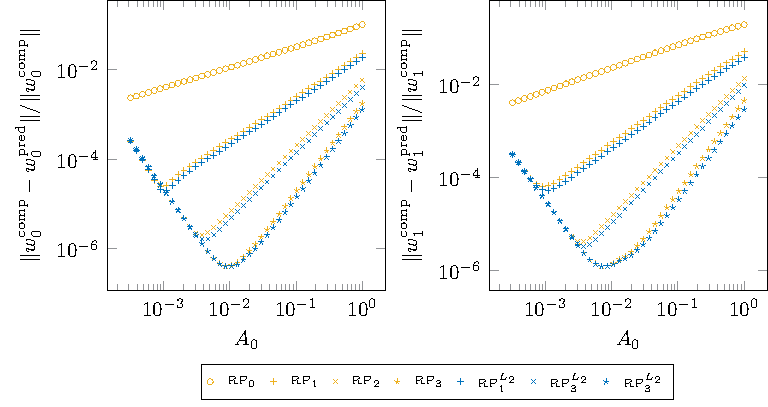
\includegraphics{\imagesdir/BTParameterdependentnormalformConvergencePlotRPMvsRPM.pdf}
    \caption{Log-log convergence plot comparing the different phase conditions
        when using the regular perturbation method (RP) for approximation the
        homoclinic solutions. The subscript in RP$_i$, $0\leq i \leq 3$, refers
        to the approximation order. The superscript $L_2$ refers to the phase
        condition \cref{eq:u_i_L2_phase_condition}. We observe here the standard V
        shaped graphs due to roundoff error.} 
    \label{fig:RP_vs_RPL2}
\end{figure}

In this example we compare five different methods to approximate the homoclinic
solution present in the universal unfolding \cref{eq:universal_unfolding}: 
\begin{itemize}
    \item the regular perturbation method, 
    \item the regular perturbation method with $L_2$ phase condition,
    \item the Lindstedt-Poincar\'e method without a higher-order time
        approximation as in~\cite{Al-Hdaibat2016},
    \item the Lindstedt-Poincar\'e method with a higher-order time
        approximation as derived here, 
    \item and the Lindstedt-Poincar\'e method with a different phase condition.
\end{itemize} 

In \cref{fig:RP_vs_RPL2} a log-log convergence plot is shown comparing the
asymptotics derived in~\cite{Al-Hdaibat2016} using the regular perturbation
method with phase condition $\dot u = 0$ against the asymptotics derived here
with the phase condition given in \cref{eq:u_i_L2_phase_condition}.  On the
abscissa is the amplitude $A_0$ and on the ordinate is the relative error
$\delta$ between the components $w_0$ and $w_1$ of the predicted solution and
the Newton corrected solution. We see that the $L_2$ phase condition is
slightly, but noticeably, more accurate at each order, confirming the geometric
intuition.

Next, we compare the regular perturbation method with the Lindstedt-Poincar\'e
method to approximate the homoclinic solution in log-log plot in
\cref{fig:RP_vs_LP2016_vs_LP}.  It is seen that the first order regular
perturbation method slightly outperforms the Lindstedt-Poincar\'e method, while
for the second and third-order the Lindstedt-Poincar\'e method  are clearly
better approximations than the regular perturbation method.  The third-order
approximation by the Lindstedt-Poincar\'e method without including a
higher-order approximation of the non-linear time transformation results in the
same order of accuracy as the zeroth-order regular perturbation method.

\begin{figure}
    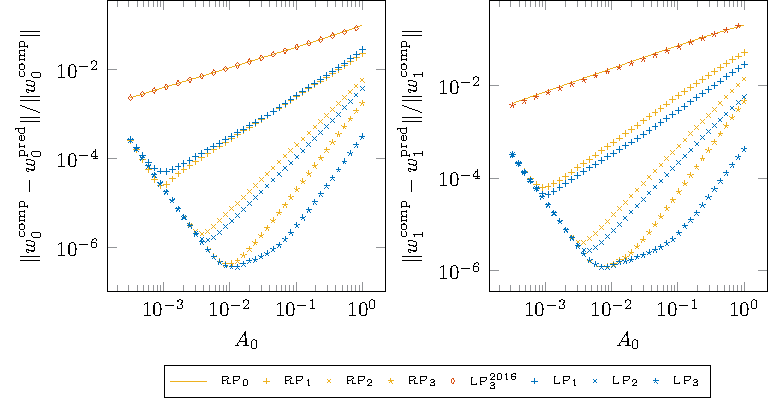
\includegraphics{\imagesdir/BTParameterdependentnormalformConvergencePlot.pdf}
    \caption{Log-log convergence plot comparing the relative errors of the computed
        homoclinic $w_0$ and $w_1$ component with the predicted solution in the
        topological normal form using four different methods: Regular
        Perturbation ($RP$, yellow), Lindstedt-Poincar\'e without higher-order time
        approximation ($LP_3^{2016}$, red), and Lindstedt-Poincar\'e combined
        with higher-order time approximation ($LP$, blue).}
    \label{fig:RP_vs_LP2016_vs_LP}
\end{figure}

It is thus essential to include a higher-order approximation of the non-linear
time transformation. To make it even more clear, we plotted the profiles of the
third-order approximations using the Lindstedt-Poincar\'e method as
in~\cite{Al-Hdaibat2016}, the regular perturbation method, and the
Lindstedt-Poincar\'e, together with the Newton corrected solutions in
\cref{fig:RP_vs_LP2016_vs_LP_profiles}. We see that the Lindstedt-Poincar\'e
method as in~\cite{Al-Hdaibat2016} approximates the solution rather poorly,
whereas the approximation derived in
\cref{sec:third_order_homoclinic_approximation_LP} is very accurate. Note that
when plotting these homoclinic approximations and corrections in $(w_0,w_1)$
phase-space, this difference is not visible at all. This explains why this has been
unnoticed in~\cite{Al-Hdaibat2016}.

\begin{figure}[!ht]
\centering
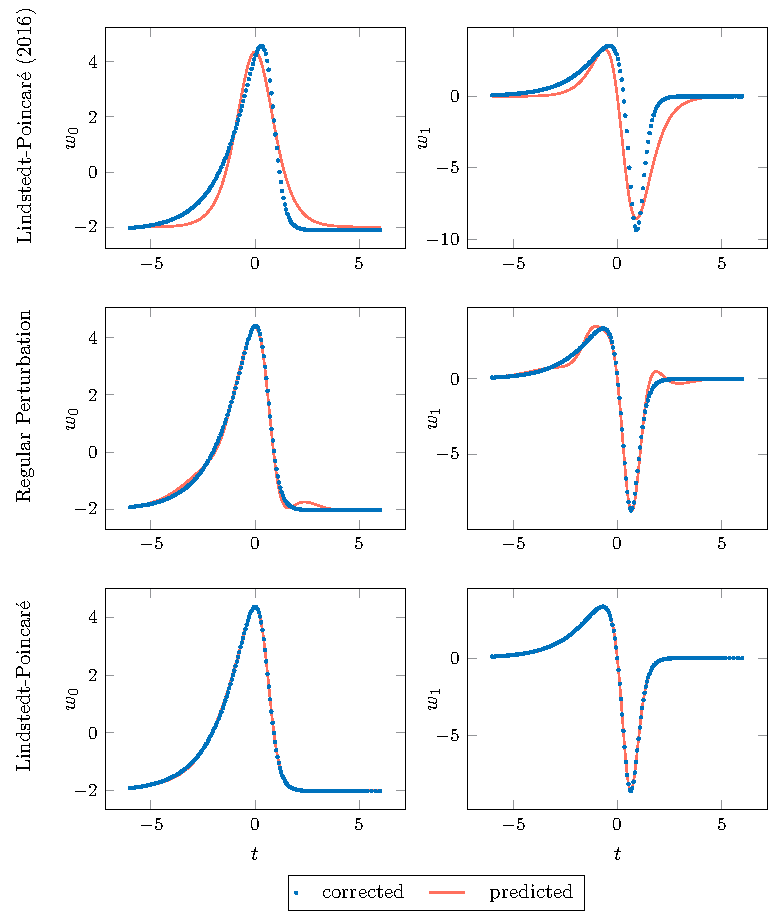
\includegraphics{\imagesdir/BTParameterdependentnormalformCompareProfiles.pdf}
\caption{Comparison of the profiles of the predicted and corrected
    homoclinic orbit for \cref{eq:universal_unfolding} using different
    approximation methods, see
\cref{sec:topological_normal_form} for a full description.}
\label{fig:RP_vs_LP2016_vs_LP_profiles}
\end{figure}

Lastly, we compare the two different phase conditions when using the
Lindstedt-Poincar\'e method in a log-log plot, in \cref{fig:LPM_vs_LPM}. It is
clearly seen that the phase condition used in \cref{sec:phase_condition}
improves, rather significantly, the accuracy of the third-order predictor.
However, in contrast with the different phase conditions used in the regular
perturbation method, we do not have any geometric (or analytical) explanation
for this improvement.

\begin{figure}
    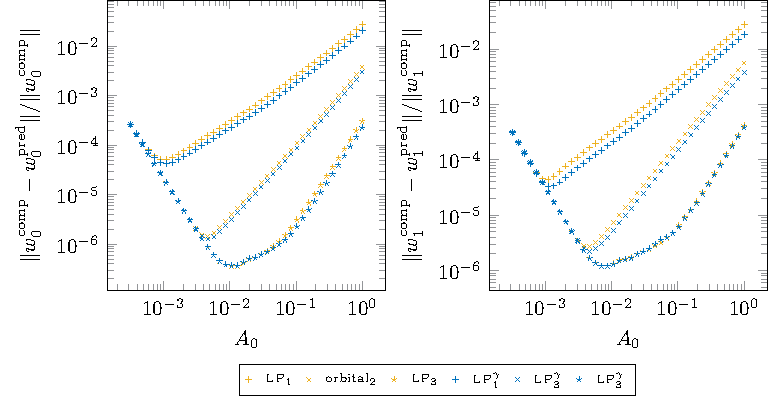
\includegraphics{\imagesdir/BTParameterdependentnormalformConvergencePlotLPMvsLPM.pdf}
    \label{fig:LPM_vs_LPM}
    \caption{
        Log-log convergence plot comparing the relative errors of the computed
        homoclinic $w_0$ and $w_1$ component with the predicted solution in the
        topological normal form using Lindstedt-Poincar\'e with two different
        phase-condition, see \cref{sec:phase_condition}.}
\end{figure}
Notice that here we do not compare the homoclinic predictors derived with
different normal forms. Indeed, when considering the universal unfolding
\cref{eq:universal_unfolding} the normal forms coincide, resulting in identical
predictors.


\subsection{Hodgking-Huxley equations}

The Hodgkin-Huxley equations~\cite{HodgkinHuxley1952} relate the difference in electric
potential across the cell membrane $V$ and gating variables $m, n$ and $h$
for ion channels to the stimulus intensity $I$ and temperature $T$, as
follows:
\begin{equation}
\label{eq:HodgkinHuxleyEquations}
\begin{cases}
\begin{aligned}
    \dot{V} &= -G(V, m, n, h)+I, \\
    \dot{m} &= \Phi(T)\left[(1-m) \alpha_{m}(V)-m \beta_{m}(V)\right], \\
    \dot{n} &= \Phi(T)\left[(1-n) \alpha_{n}(V)-n \beta_{n}(V)\right], \\
    \dot{h} &= \Phi(T)\left[(1-h) \alpha_{h}(V)-h \beta_{h}(V)\right],
\end{aligned}
\end{cases}
\end{equation}
where 
\begin{align*}
    \Phi(T) & = 3^{({T}-6.3) / 10}, \\
    G(V, m, n, h) & =\bar{g}_{\mathrm{Na}} m^{3}
    h\left(V-\bar{V}_{\mathrm{Na}}\right)+\bar{g}_{\mathrm{K}}
    n^{4}\left(V-\bar{V}_{\mathrm{K}}\right)+\bar{g}_{\mathrm{L}}\left(V-\bar{V}_{\mathrm{L}}\right).
\end{align*}
The equations modeling the variation of membrane permeability are:
\begin{align*}
    \alpha_{m}(V) =& \Psi\left(\frac{V+25}{10}\right), & \beta_{m}(V) &= 4 e^{V / 18}, \\
    \alpha_{n}(V) =& 0.1 \Psi\left(\frac{V+10}{10}\right), & \beta_{n}(V) &= 0.125 e^{V / 80}, \\
    \alpha_{h}(V) =& 0.07 e^{V / 20}, & \beta_{h}(V) &= \left(1+e^{(V+30) / 10}\right)^{-1},
\end{align*} with
\begin{equation*}
    \Psi(x) = \begin{cases}
        x /\left(e^{x}-1\right), & \text { if } x \neq 0, \\
        1, & \text { if } x=0.
    \end{cases}
\end{equation*}
The parameters $\bar{g}_{\text{ion}}$ and $\bar{V}_{\text{ion}}$ representing
maximum conductance and equilibrium potential for the ion were obtained from
experimental data by Hodgkin and Huxley, with the values given below:
\[
\begin{array}{lll}
\bar{g}_{\mathrm{Na}}=120 \mathrm{mS} / \mathrm{cm}^{2}, 
& \bar{g}_{\mathrm{K}}=36 \mathrm{mS} / \mathrm{cm}^{2}, 
& \bar{g}_{\mathrm{L}}=0.3 \mathrm{mS} / \mathrm{cm}^{2}, \\
\bar{V}_{\mathrm{Na}}=-115 \mathrm{mV},
& \bar{V}_{\mathrm{K}}=12 \mathrm{mV}, 
& \bar{V}_{\mathrm{L}}=10.599 \mathrm{mV}.
\end{array}
\]
The values of $\bar{V}_{\mathrm{Na}}$ and $\bar{V}_{\mathrm{K}}$ can be
controlled experimentally~\cite{HodgkinHuxley1952a,Jack1975ElectricCurrentFlow}.
The temperature is set to $T=6.3^{\circ}$.

It is easy to see that the equilibria of \cref{eq:HodgkinHuxleyEquations} can be
parametrized by $V$
\begin{equation*}
    \begin{aligned}
        I(V) &= G(V, m(V), n(V), h(V)) \\
        y(V) &= \alpha_y(V)/(\alpha_y(V)+\beta_y(V)),
    \end{aligned}
\end{equation*}
where $y\in\{m,n,h\}$, see also~\cite{Guckenheimer@1993}. By calculating the Jacobian $A$ of
\cref{eq:HodgkinHuxleyEquations} at the equilibrium, we can derive the
characteristic polynomial $\rho_A(\lambda)$. The equation $\rho_A(0)=0$ can be
solved analytically for $\bar V_K$. Using this solution for $\bar V_k$ and
plotting the curve $\rho'(0)$ reveals two potential candidates for Bogdanov--Takens
points. Inspecting the geometric multiplicity of these two points narrows the
possibilities down to the point
\begin{equation}
\label{eq:HodgkinHuxleyBTpoint}
\begin{pmatrix}
    V \\m \\n \\h \\ \bar V_k \\ I 
\end{pmatrix}
\approx
\begin{pmatrix}
-2.835463618170097 \\ 0.07351498630356315 \\ 0.361877602925177 \\ 0.494859128785482 \\
-4.977020454108788 \\ -0.06185214966177632
\end{pmatrix}.
\end{equation}  
Inspecting the coefficients of the normal form shows that
\[
a = 2.5515\cdot 10^{-5}, \qquad b =  -0.0075.
\] 
Thus, provided the transversality conditions are satisfied, we can use \MATCONT to
start continuation of the homoclinic orbits emanating from this point.

\begin{figure}
    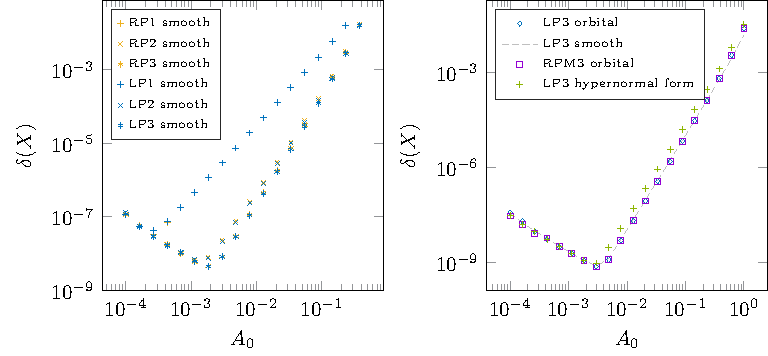
\includegraphics{\imagesdir/HodgkinHuxleyConvergencePlotFull.pdf}
    \caption{Convergence plot for the homoclinic predictors near the
    Bogdanov--Takens bifurcation \cref{eq:HodgkinHuxleyBTpoint} in the
    Hodgkin-Huxley equations \cref{eq:HodgkinHuxleyEquations}.}
    \label{fig:HodgkinHuxleyConvergencePlot}
\end{figure}

In \cref{fig:HodgkinHuxleyConvergencePlot} there are two log-log convergence
plots shown. Note that in this and the next example, we show the relative error
$\delta(X)$ between the predicted and corrected Newton solution to the defining
system \cref{eq:definingSystem}.  In the left plot (a) we compare the regular
perturbation method with the Lindstedt-Poincar\'e method. We see that compared
with the previous example, the Lindstedt-Poincare\'e method is slightly less
accurate than the regular perturbation method and the second-order.
Nevertheless, we clearly see that the order of convergence lifts from the
normal form to the two-dimensional center manifold in $\mathbb R^4$. In the
plot right (b) we compare four different third approximations to the homoclinic
orbit
\begin{itemize}
    \item the Lindstedt-Poincar\'e method using the smooth orbital normal form
        (the blue diamond),
    \item the Lindstedt-Poincar\'e method using the smooth normal form
        (the dashed light gray line),
    \item the regular perturbation method using the smooth normal form
        (the pink square), 
    \item the Lindstedt-Poincar\'e method using the hyper-normal form
        (the green plus).
\end{itemize}

We see that both the Lindstedt-Poincar\'e method and the regular perturbation
method using the smooth orbital normal form are in perfect agreement with the
Lindstedt-Poincar\'e method using the smooth normal form. Only the homoclinic
predictor using the hyper-normal form is slightly less accurate.

\subsection{Homoclinic RG flows}
In~\cite{Jepsen2021HomoclinicRG}  an $\mathcal N = 1$ supersymmetric model of interacting
scalar superfields $\Phi_{ab}^i$ that is invariant under the action of an $O(N)
\times O(M)$ group in $d = 3 - \epsilon$ dimensions is considered.
The coupling constants $g_i(i=1,\dots,4)$ satisfy the following differential
equations
\begin{equation}
    \label{eq:HomoclinicRGflows} 
    \dot g = -\epsilon g + \beta^{(2)}(g,M,N) + \mathcal O(g^5),  \qquad g\in\mathbb R^4,
\end{equation} 
where the two-loop contributions $\beta_i^{(2)}(i=1,\dots,4)$ are cubic in the
coupling and the parameter $\epsilon$ is scaled to $1$.  The exact expression for
$\beta_i^{(2)}$ are quite long can be found in~\cite[Appendix B]{Jepsen2021HomoclinicRG}
or in the Supplementary Materials. 
\begin{figure}[b!]
    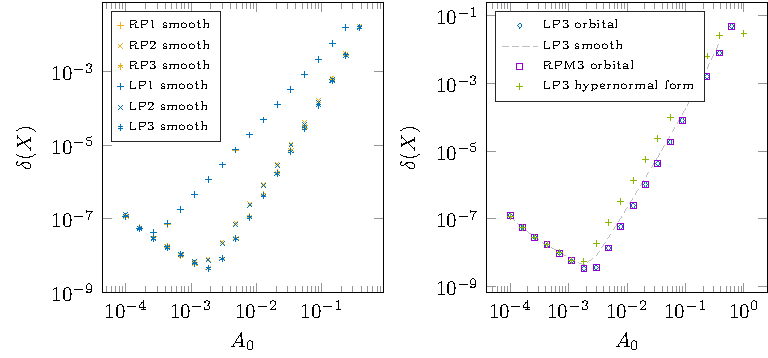
\includegraphics{\imagesdir/HomoclinicRGFlowsConvergencePlotFull.pdf}
    \caption{Convergence plot for the homoclinic predictors near one of the
        two Bogdanov--Takens bifurcation in the Homoclinic RG flows model 
        \cref{eq:HomoclinicRGflows}.}
    \label{fig:HomoclinicRGFlowsConvergencePlot}
\end{figure}
%
\begin{figure}[t!]
    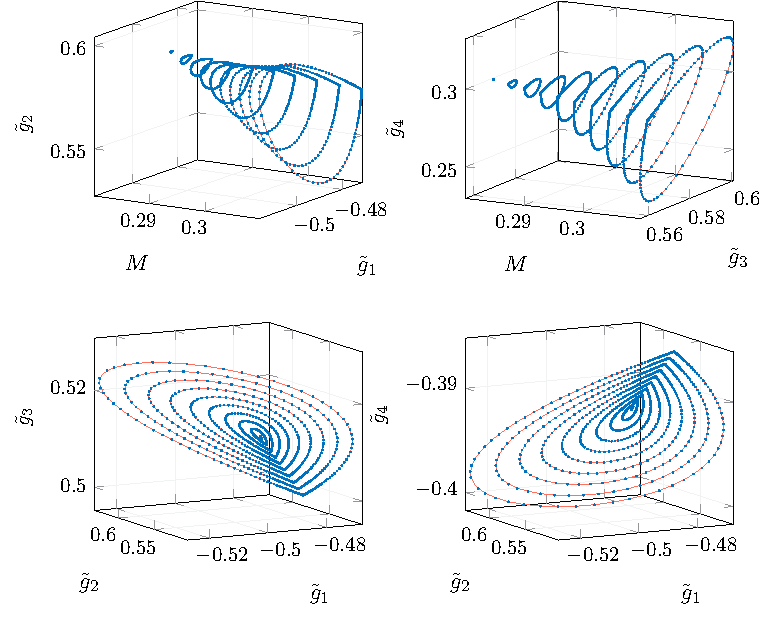
\includegraphics{\imagesdir/HomoclinicRGflowsCompareOrbits3D_LP.pdf}
    \caption{Comparison between the predicted (solid, red) with the corrected
        (dotted, blue) homoclinic orbits using the Lindstedt-Poincar\'e method
        with the smooth orbital normal form for amplitudes $A_0 = 10^{-3}$ to
        $A_0=5\times10^{-2}$. The $g_i(i=1,\dots,4)$ coordinates have been rotated and stretched
        to make the homoclinic orbits better visible.}
    \label{fig:HomoclinicRGFlows}
\end{figure}
%
\begin{figure}[t!]
\includetikzscaled{HomoclinicRGflowsCompareParameters}
\caption{Comparison between the computed homoclinic bifurcation curve
    (solid, blue) with the predicted values in parameter-space $(M,N)$.
    The yellow crosses are the second-order predictor obtained with the
    transformation as given in {\cite{Al-Hdaibat2016}}. The blue plus
    signs are the second-order predictor obtained in this paper. These are
    indistinguishable at this scale from the third-order
    predictor (dotted, red) obtained in this paper.}
\label{fig:HomoclinicRGFlowsParameters}
\end{figure}

In~\cite{Jepsen2021HomoclinicRG} a Bogdanov--Takens point near the parameter values
$M=0.2945$ and $N = 4.036$ is located. Using these parameter values we locate an
equilibrium at 
\[
\begin{pmatrix}
    g_1 \\ g_2 \\ g_3 \\ g_4
\end{pmatrix} = 
\begin{pmatrix}
    0.0701457361241472 \\ -0.06520883770451065 \\ 0.001823543197553845 \\ 0.22874527306411319
\end{pmatrix}.
\]
By continuing the equilibrium in the parameter $M$ we detect several limit
points and two Hopf points. We continue the second Hopf point at $M\approx0.2958$ 
in parameters $M$ and $N$. Several Bogdanov--Takens points are detected. The
first Bogdanov--Takens point is located at
\[
\begin{pmatrix}
    g_1 \\ g_2 \\ g_3 \\ g_4 \\ 
\end{pmatrix} = 
\begin{pmatrix}
    -0.715157316845187 \\ -0.250968103603174 \\ 0.510051114588271 \\ -0.391935453715783 \\
\end{pmatrix},
\]
with parameter values
\[
    (M, N) = (0.294477255737036, 4.035536108506390).
\]

In \cref{fig:HomoclinicRGFlowsConvergencePlot} we have created similar log-log
convergence plots as in the previous example. The plots look very alike, only
the homoclinic predictor using the hyper-normal form is in this model slightly
more accurate than the other homoclinic approximations.

Lastly, in \cref{fig:HomoclinicRGFlows}  we compare the predicted (dotted,
blue) with the corrected (solid, red) homoclinic orbits using the
Lindstedt-Poincar\'e method with the smooth orbital normal form for amplitudes
$A_0 = 10^{-3}$ to $A_0=5\times 10^{-2}$. We see that they are in excellent
agreement. In \cref{fig:HomoclinicRGFlowsParameters} we compared the computed
homoclinic bifurcation curve (solid, blue) with the predicted values in
parameter-space $(M, N)$. Most important to notice here is that the predictor
given in \cite{Al-Hdaibat2016} (the yellow crosses) is less accurate than the
second-order predictor (blue plus signs) obtained in this paper.

